%-------------------------------------------------------------------------------------
%	PACKAGES AND THEMES
%-------------------------------------------------------------------------------------
\documentclass{beamer}
\setbeamercovered{transparent}
\setbeamercolor{local structure}{fg=black}
\setbeamertemplate{caption}{\raggedright\insertcaption\par}
\usefonttheme[onlymath]{serif}

\mode<presentation> {
	
	% The Beamer class comes with a number of default slide themes
	% which change the colors and layouts of slides. Below this is a list
	% of all the themes, uncomment each in turn to see what they look like.
	
	%\usetheme{default}
	%\usetheme{AnnArbor}
	%\usetheme{Antibes}
	%\usetheme{Bergen}
	%\usetheme{Berkeley}
	%\usetheme{Berlin}
	%\usetheme{Boadilla}
	\usetheme{CambridgeUS}
	%\usetheme{Copenhagen}
	%\usetheme{Darmstadt}
	%\usetheme{Dresden}
	%\usetheme{Frankfurt}
	%\usetheme{Goettingen}
	%\usetheme{Hannover}
	%\usetheme{Ilmenau}
	%\usetheme{JuanLesPins}
	%\usetheme{Luebeck}
	%\usetheme{Madrid}
	%\usetheme{Malmoe}
	%\usetheme{Marburg}
	%\usetheme{Montpellier}
	%\usetheme{PaloAlto}
	%\usetheme{Pittsburgh}
	%\usetheme{Rochester}
	%\usetheme{Singapore}
	%\usetheme{Szeged}
	%\usetheme{Warsaw}
	
	% As well as themes, the Beamer class has a number of color themes
	% for any slide theme. Uncomment each of these in turn to see how it
	% changes the colors of your current slide theme.
	
	%\usecolortheme{albatross}
	%\usecolortheme{beaver}
	%\usecolortheme{beetle}
	%\usecolortheme{crane}
	%\usecolortheme{dolphin}
	%\usecolortheme{dove}
	%\usecolortheme{fly}
	%\usecolortheme{lily}
	\usecolortheme{orchid}
	%\usecolortheme{rose}
	%\usecolortheme{seagull}
	%\usecolortheme{seahorse}
	%\usecolortheme{whale}
	%\usecolortheme{wolverine}
	
	%\setbeamertemplate{footline} % To remove the footer line in all slides uncomment this line
	%\setbeamertemplate{footline}[page number] % To replace the footer line in all slides with a simple slide count uncomment this line
	
	%\setbeamertemplate{navigation symbols}{} % To remove the navigation symbols from the bottom of all slides uncomment this line
}

\usepackage{graphicx} % Allows including images
\usepackage{booktabs} % Allows the use of \toprule, \midrule and \bottomrule in tables
\usepackage{caption}
\captionsetup{font=scriptsize,labelfont=scriptsize}
\usepackage{amssymb}
\usepackage{bm}
%\usepackage{enumitem}
\usepackage{amsfonts}
\usepackage[colorinlistoftodos,prependcaption,textsize=small]{todonotes}
%-------------------------------------------------------------------------------------
%	TITLE PAGE
%-------------------------------------------------------------------------------------

\title[Large-Scale Data Analysis Techniques]{A Review on Multi-Label Learning Algorithms} % The short title appears at the bottom of every slide, the full title is only on the title page

\author[Sissy Themeli, Nikiforos Pittaras]{Min-Ling Zhang and Zhi-Hua Zhou} % Your name
\institute[DI-UOA] % Your institution as it will appear on the bottom of every slide, may be shorthand to save space
{
	IEEE Transactions On Knowledge And Data Engineering\\ % Your institution for the title page
	\medskip
}
\date{\today} % Date, can be changed to a custom date

\begin{document}
	
	\begin{frame}
	\titlepage % Print the title page as the first slide
\end{frame}

\begin{frame}
\frametitle{Overview} % Table of contents slide, comment this block out to remove it
\tableofcontents % Throughout your presentation, if you choose to use \section{} and \subsection{} commands, these will automatically be printed on this slide as an overview of your presentation
%\setbeamercolor{section in toc}{fg=black}
%\setbeamercolor{subsection in toc}{fg=black}
\end{frame}

%-------------------------------------------------------------------------------------
%	PRESENTATION SLIDES
%-------------------------------------------------------------------------------------

\section{Introduction} % Sections can be created in order to organize your presentation into discrete blocks, all sections and subsections are automatically printed in the table of contents as an overview of the talk
\subsection{Multi-label learning}
%------------------------------------------------
\begin{frame}
\Huge{\centerline{Introduction}}
\end{frame}
%------------------------------------------------
\begin{frame}
\frametitle{\insertsection : \insertsubsection}
Applied to supervised classification
\begin{itemize}
\item[$\bullet$] Given input data and labels, goal is to learn a model $f: X \rightarrow Y$ 
\item[$\bullet$] $f(x_i, y_i) = r$ where $r\in \mathbb{R}$ is the confidence that $y_i$ characterizes $x_i$
\item[$\bullet$] Assume that $x_i$ belongs to $y_i$ if $r \ge $ $t(x_i)$
\begin{itemize}%[label={$\checkmark$}]
\item[$\checkmark$] $t(\cdot)$ can be a predetermined constant function or learned from $X$
\end{itemize}
\end{itemize}

Single-label learning
\begin{itemize}
\item[$\bullet$] Dataset $\{ (x_i, y_i)\}, i = 1, \dots N, x \in X, y \in Y=\{y_1,\dots,y_q\}$
\end{itemize}

Multi-label learning
\begin{itemize}
\item[$\bullet$] Multi-label dataset: Multiple labels per instance. $\{ (x_i, \bm{y}_i)\}, i = 1, \dots N, x \in X, \bm{y} \in \mathbb{P}(Y)$
% \item Learn a model $f: X \times Y \rightarrow r$

\end{itemize}
%TODO: Include stuff about multi-labeled dataset characterization?
\end{frame}
%------------------------------------------------
%------------------------------------------------
\subsection{Algorithm Strategies}
\begin{frame}
\frametitle{\insertsection : \insertsubsection}
Label search space $\mathbb{S_Y}$ grows exponentially as a function of $|Y|=q$
\begin{itemize}
\item[$\triangleright$] e.g. for $q=20, |\mathbb{S_Y}| = 2 ^ {|\mathbb{P(Y)}|} = 2^{20} \ge 10^6$
\end{itemize}
Solution: integrate in the learning process potential label correlations.
This work examines algorithms grouped in three broad categories:

\begin{enumerate}
\item First-order strategies
\begin{itemize}
\item[$\circ$] Ignore label correlations
\item[$\circ$] Often transform M-L problem to multiple, single-label problems
\item[$\circ$] Simple, scalable, suboptimal
\end{itemize}
\item Second-order strategies
\begin{itemize}
\item[$\circ$] Consider \emph{pairwise} label relations
\item[$\circ$] Good trade-off between generalization performance and scalability
\item[$\circ$] Lacking in some real-world applications
\end{itemize}
\item Higher-order strategies
\begin{itemize}
\item[$\circ$] Capture more complicated label interdependencies
\item[$\circ$] Strong modeling capabilities
\item[$\circ$] Computationally demanding, less scalable
\end{itemize}

\end{enumerate}
\end{frame}

%------------------------------------------------
\subsection{Evaluation Metrics}
\begin{frame}
\frametitle{\insertsection : \insertsubsection}
Extension of single-label metrics to the M-L case.

Two categories and perspectives:
\begin{itemize}
\item[$\bullet$] \emph{Example-based: }Evaluates multi-labeled performance on each example, extrapolate to whole dataset
\begin{itemize}
\item[$\circ$] \emph{Classification perspective:}
\begin{itemize}
\item[$\star$] Subset Accuracy, Hamming Loss
\item[$\star$] Precision, Recall, F-measure, F$^\beta$ -measure
\end{itemize}
\item[$\circ$] \emph{Ranking perspective:} one-error, coverage, ranking loss, average precision
\end{itemize}
\item[$\bullet$] \emph{Label-based: }Evaluates performance on each label separately, extrapolate to whole label set
\begin{itemize}
\item[$\circ$] Classification perspective: Macro/Micro averaging for single-label example-based, classification-based measures
\item[$\circ$] Ranking perspective: Macro/Micro averaging for AUC
\end{itemize}
\end{itemize}
$\ast$ Classifiers should aim to optimize \emph{multiple} metrics
\end{frame}
%------------------------------------------------
\section{Multi-label Learning Algorithms}
%------------------------------------------------
\subsection{Categorization}
%------------------------------------------------
\begin{frame}
\Huge{\centerline{Multi-label Learning Algorithms}}
\end{frame}
%------------------------------------------------
\begin{frame}
\frametitle{\insertsection : \insertsubsection}

Group algorithms in two categories:
\begin{itemize}
\item[$\bullet$] \emph{Problem Transformation Methods:}

\begin{itemize}
\item[$\circ$] Transform the learning problem into other well-established learning scenarios
\item[$\circ$] ``Fit data to algorithm'' philosophy
\end{itemize}

\item[$\bullet$] \emph{Algorithm Adaptation Methods:}
\begin{itemize}
\item[$\circ$] Adapt popular learning techniques to deal with multi-label data directly
\item[$\circ$] ``Fit algorithm to data'' philosophy
\end{itemize}
\end{itemize}

Include algorithms that:
\begin{itemize}
\item[$\checkmark$] Has broad, noteworthy or unique characteristics
\item[$\checkmark$] Has primitive impact, i.e. leads to a number follow-up related methods
\item[$\checkmark$] Is influential and highly-cited in multi-label learning
\end{itemize}

\end{frame}
%------------------------------------------------
\subsection{Problem Transformation Methods}
%------------------------------------------------
\begin{frame}
\Huge{\centerline{Problem Transformation Methods}}
\end{frame}
%------------------------------------------------
\begin{frame}
\frametitle{\insertsection : \insertsubsection}
\begin{figure}
\begin{center}
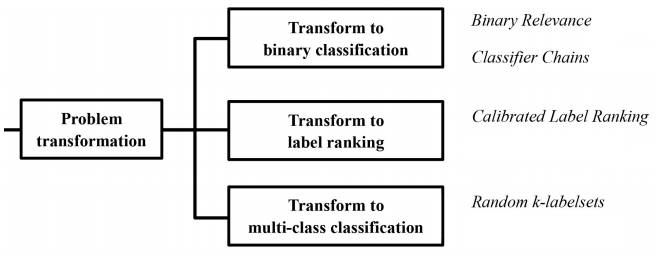
\includegraphics[scale = 0.7]{images/pt.png}
\end{center}
\end{figure}
\end{frame}
%------------------------------------------------
\begin{frame}
\frametitle{Binary Relevance}

\begin{itemize}
\item[$\bullet$] Decompose multi-label problem to $q$ independent binary classification problems
\item[$\bullet$] Construct $q$ binary (one-vs-all) training sets (one for each $y_i$)
\item[$\bullet$] Cross-train each binary classifier $h_i(x)$ on its respective dataset

\item[$\bullet$] Predict labels of an unseen $x$ by evaluating each classifier $h_i(x)$
\item[$\bullet$] Assign label $y_i$ according to $h_i(x)$ and the thresholding/ranking scheme 
\end{itemize}

Pros \& cons:
\begin{itemize}
\item[$\bullet$] Simple, one-vs-rest scheme, parallelizable
\item[$\bullet$] Sensitive to class-imbalanced data
\item[$\bullet$] Ignores label correlations (first-order method)
\end{itemize}

\end{frame}
%------------------------------------------------

\begin{frame}
\frametitle{Classifier chains}
\begin{itemize}
\item[$\bullet$] A permutation function $f_p$ is used to order $Y$
\item[$\bullet$] Transform into a \emph{chain} of binary classification problems
\item[$\bullet$] Enrich representations at step $j$ by concatenating each $x_i$ with the confidence of preceeding $1,\dots,j-1$-th classifiers
\item[$\bullet$] Predict relevant labels for unknown instances by iteratively traversing the classifier chain
\item[$\bullet$] $\lambda_{\tau(j)}^x \in \{-1,+1\}$ represents the predicted binary assignment
of $y_{\tau(j)}$, which is recursively obtained
\end{itemize}

Pros \& cons:
\begin{itemize}
\item[$\bullet$] High-order method: exploitation of label correlations to a degree, but in a random manner
\item[$\bullet$] Highly sensitive to $f_p$. Ensemble schemes attempt to overcome it.
\item[$\bullet$] Iterative operation prevents parallel implementation
\end{itemize}
\end{frame}
%------------------------------------------------

\begin{frame}
\frametitle{Calibrated Label Ranking}
\begin{itemize}
\item[$\bullet$] Transform into a label pairwise comparison ranking problem
\item[$\bullet$] For $q$ labels, generate $q(q-1)/2$ binary classifiers by pairwise comparison and use a binary algorithm $g_{jk}(x)$
\item[$\bullet$] Construct training sets $D_{jk} : \{x_i, Y_i | y_j \in Y_i \oplus y_k \in Y_i\}$. System votes for each example and if $g_{jk}(x) >0$,$x_i$ is associated with $y_j$, otherwise with $y_k$
\item[$\bullet$] For an unknown instance, all classifiers' votes are aggregated and ranked
\item[$\bullet$] A virtual label $y_v$ serves as the artificial splitting point between relevant and irrelevant labels
\end{itemize}
Pros \& cons:
\begin{itemize}
\item[$\bullet$] Second-order approach algorithm. One-vs-one scheme.
\item[$\bullet$] Smooths out the class-imbalance problem
\item[$\bullet$] Number of classifiers s quadratic to $|Y|$ (compared to linear for BR)
\begin{itemize}
\item[$\circ$] Pruning methods to reduce the search space
\end{itemize}
\end{itemize}
\end{frame}
%------------------------------------------------
\begin{frame}
\frametitle{Random k-Labelsets}
\begin{itemize}
\item[$\bullet$] Decompose to an ensemble of multi-class classification problems
\item[$\bullet$] Each component targets a random subset of $\mathbb{P}(Y)$ that appears in $X$, classified with Label Powerset (LP) techniques:
\begin{itemize}
\item[$\circ$] Transform to single-label data by treating each distinct labelset as a new class
\item[$\circ$] Each example is reassigned with the new mapped class and classified through regular single-label classification
\item[$\circ$] M-L classify $x$ with $y_i$ when the votes received for $y_i$ from the ensemble exceed half the max possible it can get
\end{itemize}
todo how does each LP classify, k-labelsets
\end{itemize}
Pros \& cons:
\begin{itemize}
\item[$\bullet$] High-order approach algorithm
\item[$\bullet$] Data-sensitive: Cannot generalize to labelsets not in the training set, too few examples for some labelsets
\item[$\bullet$] Large $Y$ implies high training complexity.
\item[$\bullet$] Improve by invoking an ensemble on random k-sized labelsets
\end{itemize}
\end{frame}
%------------------------------------------------
\subsection{Alogrithm Adaptation Methods}
%------------------------------------------------
\begin{frame}
\Huge{\centerline{Algorithm Adaptation Methods}}
\end{frame}
%------------------------------------------------
\begin{frame}
\frametitle{\insertsection : \insertsubsection}
\begin{figure}
\begin{center}
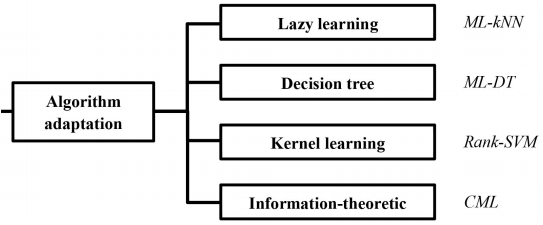
\includegraphics[scale = 0.75]{images/aa.png}
\end{center}
\end{figure}
\end{frame}
%------------------------------------------------
\begin{frame}
\frametitle{Multi-Label k-Nearest Neighbour}
\begin{itemize}
\item[$\bullet$] First-order approach algorithm, adapting knn techniques
\item[$\bullet$] Compares the MAP probabilities: $P(K|C_j), K \in \{H_j, \neg H_j\}$
\item[$\bullet$] Priors $P(K)$ computed by smoothed frequency estimation in the training data
\item[$\bullet$] Likelihoods $P(C_j|K)$ are computed as a function of:
\begin{itemize}
\item[$\circ$] $\kappa(r)$, the number of examples labelled $y_j$ with $r$ neighbours labelled $y_j$
\item[$\circ$] $\overset{\sim}{\kappa}(r)$, the number of examples not labelled $y_j$ with $r$ neighbours labelled $y_j$
\end{itemize}
\end{itemize}

Pros \& cons:
\begin{itemize}
\item[$\bullet$] First-order approach, Bayesian and Lazy reasoning
\item[$\bullet$] Decision boundary can be modified on-line via new instances
\item[$\bullet$] Class imbalance can be overcome by calculating priors
\item[$\bullet$] Extensions proposed for label correlation exploitations
\end{itemize}


\end{frame}
%------------------------------------------------
\begin{frame}
\frametitle{Multi-label Decision Tree}
\begin{itemize}
\item[$\bullet$] Multi-label entropy is used to build a decision tree recursively
\item[$\bullet$] Split position is such that the information gain criterion is maximized
\item[$\bullet$] Dataset $T$ is split on the $l$-th feature valued $\theta$ to branches ($T^-$ \& $T^+$), where $ x_{il} \leq \theta, x_i \in T^-$ and $ x_{il} > \theta, x_i \in T^+$
\item[$\bullet$] Recurse on subtrees until a stopping criterion is met (e.g. child size)
\item[$\bullet$] Single-label entropy is computed by considering labelsets as new classes
\item[$\bullet$] Assumes independence among labels to ensure low computational cost
\item[$\bullet$] Unseen instances are assigned the label of the majority of members of the leaf they arrive
\end{itemize}
Pros \& cons:
\begin{itemize}
\item[$\bullet$] First-order algorithm, highly efficient
\item[$\bullet$] Assumes label independence
\item[$\bullet$] Pruning and ensemble strategies proposed
\end{itemize}
\end{frame}
%------------------------------------------------
\begin{frame}
\frametitle{Ranking Support Vector Machine}
\begin{itemize}
\item[$\bullet$] $q$ linear classifiers, optimized to minimize the empirical ranking loss
\item[$\bullet$] For each relevant-nonrelevant label pair $(y_j,y_k) \in Y_j \times \bar Y$ their decision boundary is marked by $\left<w_j,w_k\right> + b_j - b_k=0$
\item[$\bullet$] Retrieves a ranked label pairs list for each unseen instance
\item[$\bullet$] Non-linearity achievable through feature mapping and the kernel trick
\item[$\bullet$] Convex quadratic programming problem, solved by any QP solver
\end{itemize}
Pros \& cons:
\begin{itemize}
\item[$\bullet$] Second-order approach, maximum margin strategy
\item[$\bullet$] Extensible by kernel learning, kernel selection can be overcome by MKL techniques
\item[$\bullet$] Adaptable learning by selecting an appropriate loss function
\end{itemize}

\end{frame}
%------------------------------------------------
\begin{frame}
\frametitle{Collective Multi-Label Classifier}
\begin{itemize}
\item[$\bullet$] Labels encoded as binary random vectors into a joint pdf
\item[$\bullet$] Label correlations encoded into the joint pdf as constraints
\item[$\bullet$] Model via the maximum information entropy criterion: $H_p(x, y)$, subject to constraints $\mathbb{E_p}[f_k(x,y)] = F_k$, where $F_k$ are estimated from the training set
\item[$\bullet$] Objective arrived by Lagrange multipliers, solvable by any constraint optimization solver
\item[$\bullet$] Unseen instances labelled with $Y = \underset{y}{\text{argmax }} P(y | x)$
\end{itemize}
Pros \& cons:
\begin{itemize}
\item[$\bullet$] Second-order approach. All label pairs considered, not just relevant-irrelevant ones.
\item[$\bullet$] Intractable $\text{argmax}$ operation for a large label space without pruning.
\end{itemize}
\end{frame}
%------------------------------------------------
\begin{frame}
\frametitle{\insertsection : Summary}
\begin{figure}
\begin{center}
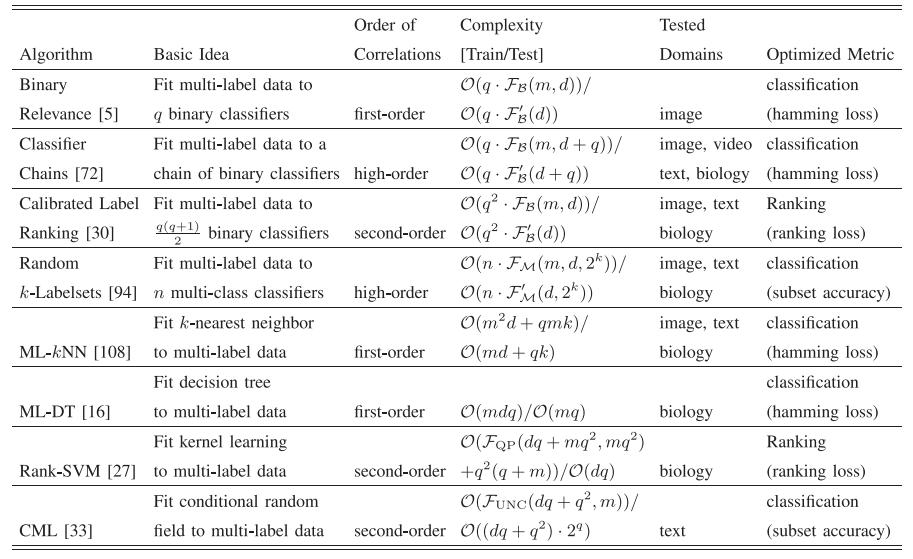
\includegraphics[scale = 0.45]{images/summary.png}
\caption{Summary of Representative Multi-Label Learning Algorithms}
\end{center}
\end{figure}
\end{frame}
%------------------------------------------------
\section{Related Learning Settings}
%------------------------------------------------
\begin{frame}
\frametitle{\insertsection}
\begin{itemize}
\item[$\bullet$] Multi-instance learning
\begin{itemize}
\item[$\circ$] Each ML example described by a bag of instances while associated with a single/binary label
\item[$\circ$] Models the object’s complex semantics in input space, rather than its output
\end{itemize}
\item[$\bullet$] Ordinal classification
\begin{itemize}
\item[$\circ$] Model class co-relevance in a (vague) graded membership vector
\item[$\circ$] Transform ML problem to a set of ordinal set of problems
\end{itemize}
\item[$\bullet$] Multi-task learning
\begin{itemize}
\item[$\circ$] Multiple tasks trained in parallel, sharing information
\item[$\circ$] Knowledge from related tasks used as an inductive bias to improve generalization
\item[$\circ$] Shared or different feature space, small task workload
\end{itemize}
\item[$\bullet$] Data streams classification
\begin{itemize}
\item[$\circ$] Real-world objects are generated online and processed in  real-time
\item[$\circ$] Concept drift problem
\end{itemize}
\end{itemize}
\end{frame}

%------------------------------------------------
\section{Conclusion}
%------------------------------------------------
\begin{frame}
\Huge{\centerline{Conclusion}}
\end{frame}
%------------------------------------------------
\begin{frame}
\frametitle{\insertsection : Online resources}
\begin{figure}
\begin{center}
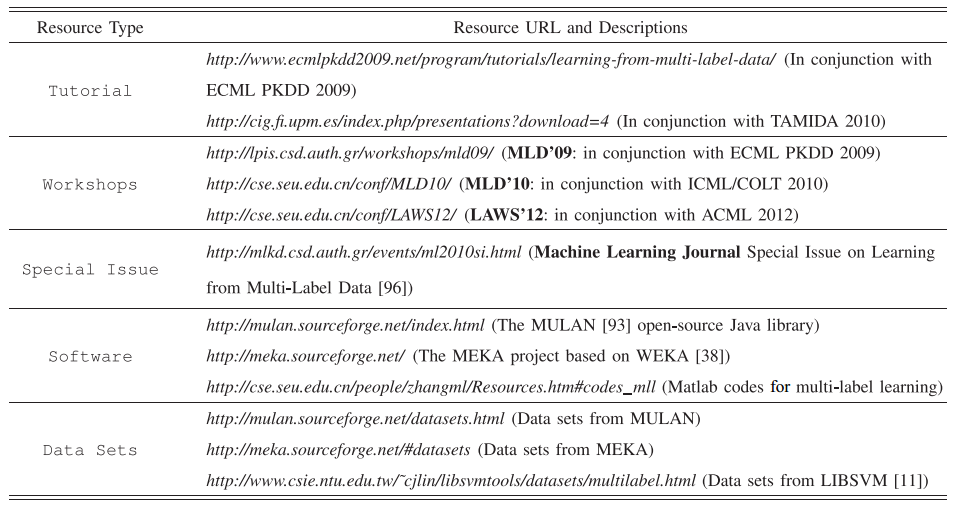
\includegraphics[scale = 0.47]{images/online.png}
\caption{Online Resources for Multi-Label Learning}
\end{center}
\end{figure}
\end{frame}
%------------------------------------------------
\begin{frame}
\frametitle{\insertsection}
Summary:
\begin{itemize}
\item[$\bullet$] Multi-label learning problem definition
\item[$\bullet$] Multi-label learning representative algorithms
\item[$\bullet$] Related learning settings
\end{itemize}

Future goals:
\begin{itemize}
\item[$\bullet$] Holy grail: Formal characterization on the underlying concept / mechanism on the appropriate usage of label correlations, especially on large output spaces
\item[$\bullet$] Thorough experimental comparative study to discover pros and cons of different multi-label learning algorithms
\end{itemize}
\end{frame}

%------------------------------------------------
\subsection{Related Work}
\begin{frame}
\frametitle{\insertsection : \insertsubsection}
\begin{itemize}
\item[$\bullet$] Madjarov, Gjorgji, et al. "An extensive experimental comparison of methods for multi-label learning." Pattern Recognition 45.9 (2012): 3084-3104
\item[$\bullet$] Tsoumakas, Grigorios, and Ioannis Katakis. "Multi-label classification: An overview." International Journal of Data Warehousing and Mining 3.3 (2006)
\item[$\bullet$] Zhang, Min-Ling, and Kun Zhang. "Multi-label learning by exploiting label dependency." Proceedings of the 16th ACM SIGKDD international conference on Knowledge discovery and data mining. ACM, 2010
\end{itemize}
\end{frame}

%------------------------------------------------
\section{The end}
\begin{frame}
\Huge{\centerline{Thank you}}
\Huge{\centerline{Questions?}}
\end{frame}
%------------------------------------------------
\end{document}
